\subsubsubsubsection{Street Director}
\begin{figure}[h]
\centering
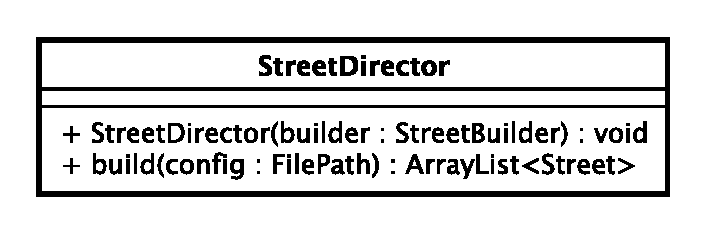
\includegraphics[scale=0.6,keepaspectratio]{images/solution/street_director.eps}
\caption{App::Reactive::Street Director}
\label{fig:sd-app-street_director}
\end{figure}
\FloatBarrier
\begin{itemize}
  \item \textbf{Description} \\
    It represents the concrete director of the street builder.
  \item \textbf{Operation}
  \begin{itemize} 
    \item \texttt{+ StreetDirector(builder: StreetBuilder)} \\
Creates a concrete street director with its own street builder.
    \item \texttt{+ build(config: FilePath) : ArrayList<Street>} \\
Builds a list of streets according to the configuration file. 
It uses the builder multiple times to create incrementally a 
specific configuration of the requested street specified 
in the configuration file. 
  \end{itemize}
\end{itemize}
